\part{Using LabPlot}

\chapter{Interface}\label{ch:interface}
\section{Main Area}\label{sec:main_area}
\section{Project Explorer}\label{sec:project_explorer}
\section{Properties Explorer}\label{sec:properties_explorer}
\section{Worksheet}\label{sec:worksheet}

\chapter{Data Containers}\label{ch:data_container}
\section{Spreadsheet}\label{sec:spreadsheet}
The spreadsheet is the main part of LabPlot when working with data and consists of columns.
Column is the basic data set in LabPlot used for plotting and data analysis.
Every column of the spreadsheet is specified by its name and the type - numeric, text, month names, day names and date and time.
Also, for each type different representation formats can be assigned like decimal or scientific format for numeric columns etc.

You can mask selected data points in the spreadsheet (\menuchoice{Selection}{Mask Selection} from the spreadsheet cell context menu).
Masked data is not plotted and is also excluded from data analysis functions like fitting etc.
Alternatively, you can mask or drop values in a column (\menuitem{Mask Values} or \menuitem{Drop Values} from the column context menu) by specifying a range.
When specifying which values to mask or to drop, several operators (“equal to”, “greater than”, “lesser than”, etc.) are available.
These operations can help to hide or to remove some outliers in the data set prior to, e.g., performing a fit to this data set.

Any spreadsheet function can be reached via the context menu (\rmb).
You can cut, copy and paste between spreadsheets, generate, normalize and sort data and finally make plots out of your data.
\begin{figure}
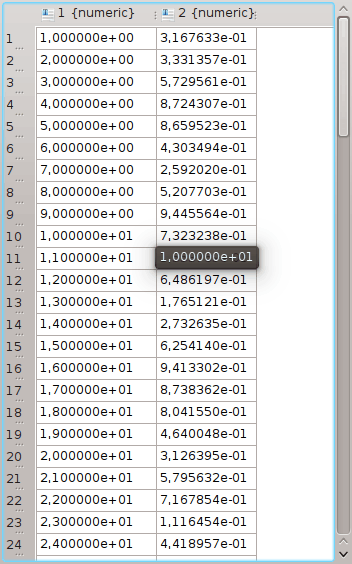
\includegraphics[width=\textwidth]{images/spreadsheet.png}
\caption{Spreadsheet showing some imported data.}
\end{figure}

New data can be produced either by entering it manually in the spreadsheet or by generating the data according to a certain prescription.
LabPlot provides 5 different methods to generate data, accessible via the context menu of the column:
\begin{itemize}
\item \textbf{Row Numbers} - values in the column are set according to its row number, this provide an easy way to quickly create an index.
%
\item \textbf{Constant Values} - values in the column are set to a constant value provided by the user.
%
\item \textbf{Equidistant values} (for numeric columns only) - given the minimal and the maximal values, the equidistant values can be either generated
by fixing the total number of values in that range or by fixing the increment (distance).
%
\item \textbf{Random values} (for numeric columns only) - values are randomly generated according to the selected distribution.
To generate uniformly distributed random numbers, select "Flat" distribution.
In the simplest cases a non-uniform distribution is calculated analytically from the uniform distribution of a random number generator by applying
an appropriate transformation. More complicated distributions are created by the acceptance-rejection method, which compares the desired distribution
against a distribution which is similar and known analytically.
%
\item \textbf{Function values} (for numeric columns only) - values are generated according to a mathematical function provided by the user,
a column (data set) containing the function arguments has to be provided.
It is possible to define a multivariant function and to provide a data set (a column in a spreadsheet) for each of the variables.
The corresponding dialog supports the creation of arbitrary number of variables
\end{itemize}

% TODO
% \begin{figure}
% 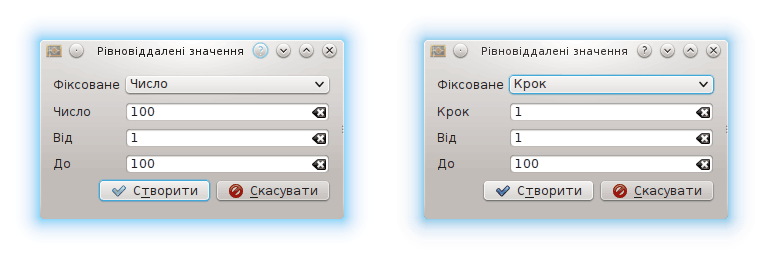
\includegraphics[width=\linewidth]{images/spreadsheet_generate_equidistant_values.png}
% \caption{Dialog for generating equidistant numbers}
% \end{figure}
% \begin{figure}
% 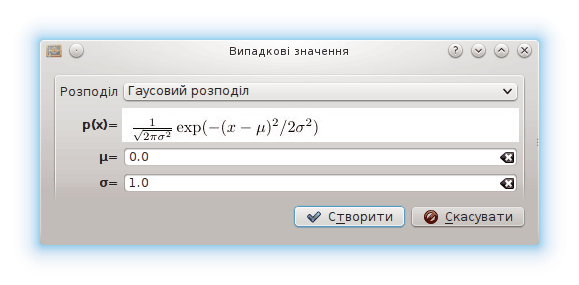
\includegraphics[width=\linewidth]{images/spreadsheet_generate_random_values.png}
% \caption{Dialog for generating equidistant numbers}
% \end{figure}
% \begin{figure}
% 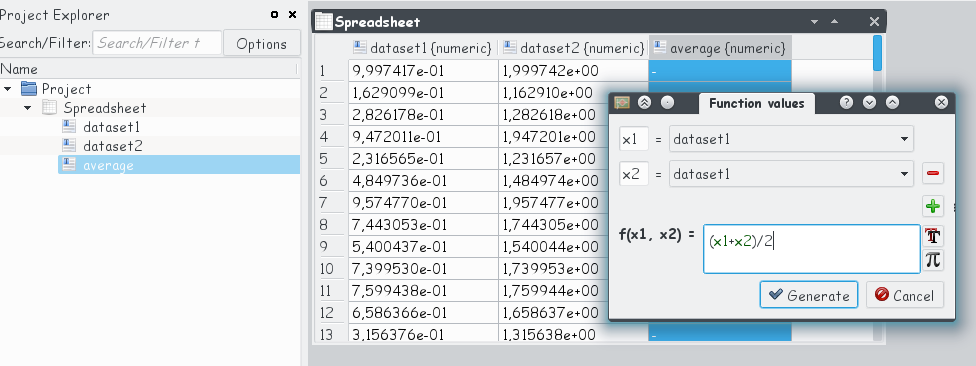
\includegraphics[width=\linewidth]{images/spreadsheet_generate_multivariant_function_values.png}
% \caption{Dialog for generating equidistant numbers}
% \end{figure}

Already existing data can be imported into a spreadsheet from external files via the "Import Data" dialog (s.a. \nameref{sec:import}).
Imported data will be stored in the project file. Changes on data, performed either in the spreadsheet or in the external file after the import, are not synchronized anymore.

The data in the spreadsheet can be exported to an external file (s.a. \nameref{sec:export}).



\section{Matrix}\label{sec:matrix}
Matrix is another container for matrix-like data. This container is presented like a table or, alternatively, as a two-dimensional greyscale image.
The elements of such a table/matrix can be thought as being the$z$-values, $z=z(x,y)$, with $x$ and $y$ values being the row and column numbers, respectively.
The transition from the row and column numbers to the logical coordinates is done via an explicit user-defined mapping of both representations.
\begin{figure}
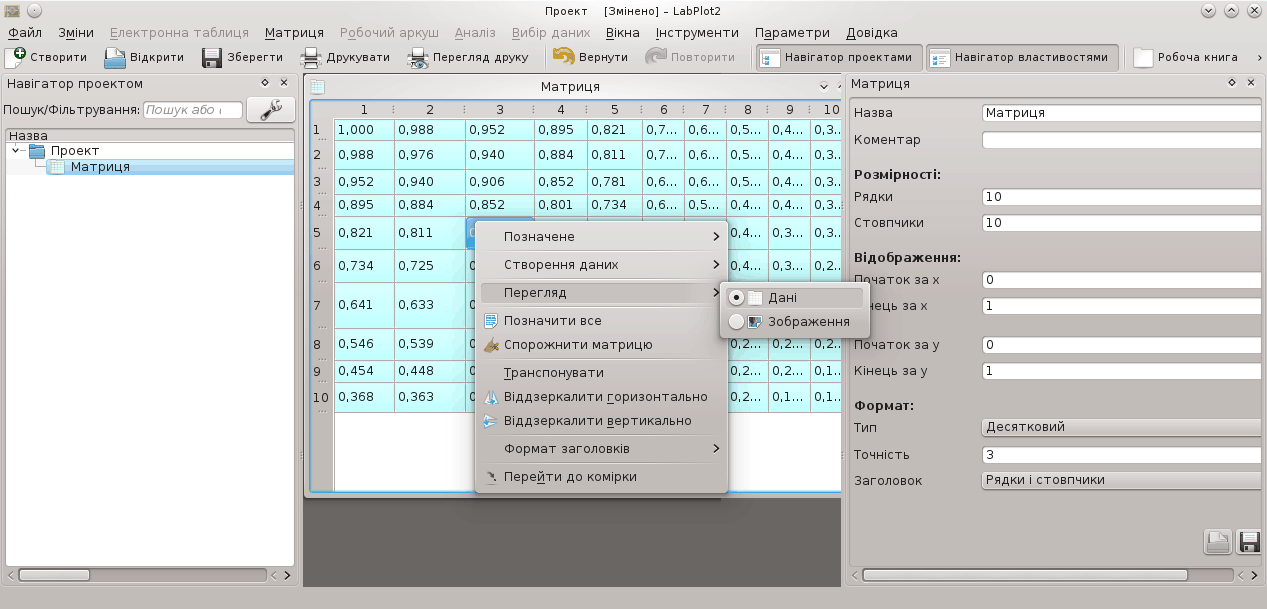
\includegraphics[width=\textwidth]{images/matrix.png}
\caption{Matrix with 500x500 values in the ranges $x=[0,1]$ and $y=[0,1]$. The cell values, $z$, are given by $z=z(x,y)$.}
\end{figure}

The matrix data can either be entered manually or via an import from an external file.
Similar to the data generation for a column in a \nameref{sec:spreadsheet}, the matrix can be filled with constant values or via a formula, too.
% TODO
% \begin{figure}
% 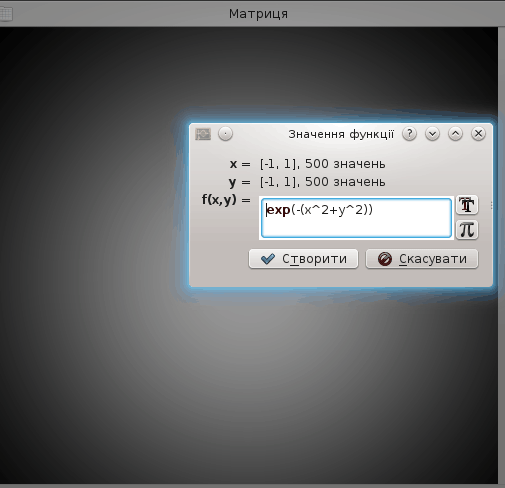
\includegraphics[width=\textwidth]{images/matrix_function_values.png}
% \caption{Image view of a matrix together with the formula that was used to generate the matrix elements}
% \end{figure}

%TODO: export matrix to different formats

\section{Workbook}\label{sec:workbook}
Workbook helps the user to better organize and to group different data containers (Spreadsheet and Matrix).
This object serves as the parent container for multiple Spreadsheet- and/or Matrix-objects and puts them together in a view with multiple tabs.
\begin{figure}
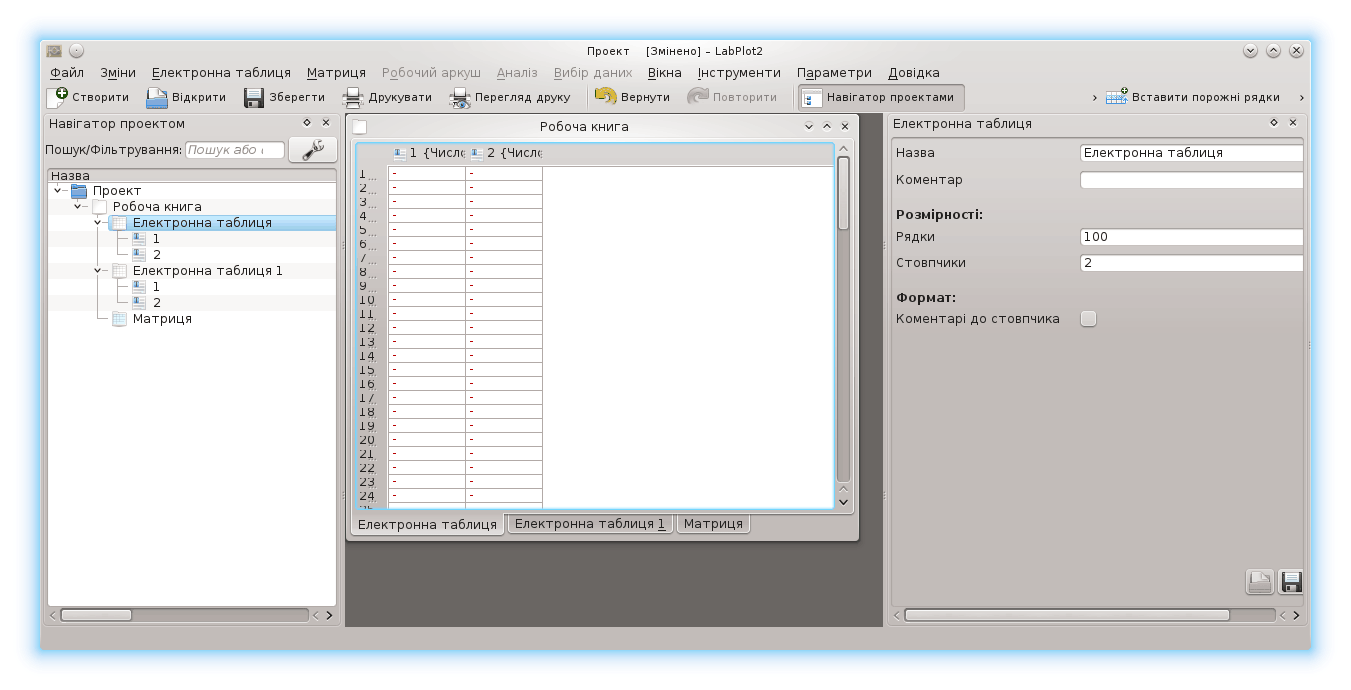
\includegraphics[width=\textwidth]{images/workbook.png}
\caption{Workbook combining two spreadsheets and one matrix in one container.}
\end{figure}

With folders it is already possible to bring some structure in the \nameref{sec:project_explorer} and to group together several related objects
(spreadsheets with data stemming from text files of similar origin, red, green and blue values of an image imported into three different matrices, etc.).
With Workbook the user has the possibility for another additional grouping.


\chapter{2D Plotting}\label{ch:2d_plotting}
\section{Plots}\label{sec:2d_plots}
\section{Curves}\label{sec:2d_curves}
\section{Legends}\label{sec:2d_legends}


% \chapter{3D Plotting}

\chapter{Themes and Templates}\label{ch:themes_templates}


\chapter{Data Analysis}\label{ch:data_analysis}
\section{Data reduction}\label{sec:data_reduction}
\section{Differentiation}\label{sec:differentiation}
\section{Integration}\label{sec:integration}
\section{Interpolation}\label{sec:interpolation}
\section{Smoothing}\label{sec:smoothing}
\section{Curve Fitting}\label{sec:curve_fitting}
LabPlot calculates several statistical measures that help to estimate the goodness of the fit.

\textbf{Sum of squared errors (SSE)} (also known as residual sum of squares (RSS) or sum of squared residuals (SSR)):
\begin{eqnarray*}
SSE = \sum_{i=1}^n (\bar y -y)^2.
\end{eqnarray*}
\textbf{Mean squared error (MSE):}
\begin{eqnarray*}
MSE = \frac{1}{n} \sum_{i=1}^n (\bar y -y)^2.
\end{eqnarray*}
\textbf{Root-mean squared error (RMSE):}
\begin{eqnarray*}
RMSE = \sqrt{MSE}.
\end{eqnarray*}
\textbf{Mean absolute error (MAE):}
\begin{eqnarray*}
MAE = \frac{1}{n} \sum_{i=1}^n |\bar y -y|^2.
\end{eqnarray*}
\textbf{Residual mean square (RMS):}
\begin{eqnarray*}
RMS = \frac{SSE}{n-p}.
\end{eqnarray*}
\textbf{Residual standard deviation (RSD):}
\begin{eqnarray*}
RSD = \sqrt{RMS}
\end{eqnarray*}
\textbf{Coefficient of determination ($\mathbf{R^2}$):}
\begin{eqnarray*}
R^2 = 1 - \frac{SSE}{TSS},\; \text{with the total sum of squares}\; TTS = \sum_i (y_i - \hat y)^2\; \text{and}\; \hat y = \frac 1n \sum_{i=1}^n y_i.
\end{eqnarray*}
\textbf{Adjusted coefficient of determination (}$\mathbf{R^2_{Adj.}}$\textbf{):}
\begin{eqnarray*}
R^2_{\mathrm{Adj.}} = 1 - \frac{SSE/(n-1)}{TSS/(n-p-1)} =  1 - (1-R^2) \frac{n-1}{n-np-1}.
\end{eqnarray*}


The implementation of the fitting procedure with bounded parameters follows the implementation in MINUIT (http://seal.web.cern.ch/seal/documents/minuit/mnusersguide.pdf, Sec. 1.3.1). Using hard limits for the parameters directly during the calculation is hard to accomplish, especially while calculating the derivatives. Instead of this, a transformation to internal parameters that are free from any bounds is performed. This transformation is constructed in such a way as to limit the original (external) parameters to the specified bounds while allowing the internal parameters to take any values.

For both, the lower ($\min$) and the upper ($\max$) parameter bounds specified, the mapping between the bounded parameters and the parameters used internally in the calculation is given by
\begin{eqnarray*}
P_{int} &=& \arcsin \left( 2\frac{P_{ext} - \min}{\max - \min} - 1 \right), \\
P_{ext} &=& \min + \frac{\max - \min}{2} \left( \sin P_{int} + 1 \right).
\end{eqnarray*}
For single sided limits with only the lower limit available:
\begin{eqnarray*}
P_{int} &=& \pm \sqrt{ (P_{ext} - \min + 1)^2 - 1}, \\
P_{ext} &=& \min - 1 + \sqrt{P_{int}^2 + 1}.
\end{eqnarray*}
And similarly for parameters with upper limits only:
\begin{eqnarray*}
P_{int} &=& \pm \sqrt{ (\max - P_{ext} + 1)^2 - 1},\\
P_{ext} &=& \max + 1 - \sqrt{P_{int}^2 + 1}.
\end{eqnarray*}
The transformation is non-linear which introduces, even for linear problems, additional non-linearity and numerical instabilities. Therefore, it is recommended to impose limits on the parameters only if really required. Furthermore, in order to get more stable error analysis results the fit should be re-performed again without any limits once a reasonable minimum was found.

\section{Fourier Filter}\label{sec:fourier_filter}

\newpage
\section{Fourier Fransform}
Available window functions are
\begin{eqnarray*}
\text{rectangular(uniform):} \quad  w(n) &=& 1 \\
\text{triangular:} \quad w(n) &=& 1 - \frac{2}{N} \left| n-\frac{N-1}{2} \right| \\
\text{triangular (Bartlett):} \quad  w(n) &=&  1 - \frac{2}{N-1} \left|n-\frac{N-1}{2}\right| \\
\text{triangular (Parzen):} \quad  w(n) &=& 1 - \frac{2}{N+1} \left| n-\frac{N-1}{2} \right| \\
\text{Welch (parabolic):} \quad  w(n) &=& 1 - \left(2 \frac{n-(N-1)/2}{N+1} \right)^2 \\
\text{Cosine:} \quad  w(n) &=& \sin\left( \frac{\pi n}{N-1} \right) \\
\text{Bartlett-Hann:} \quad  w(n) &=& 0.62 - 0.48 \left| \frac{n}{N-1}-0.5 \right| - 0.38 \cos\left(\frac{2\pi n}{N-1}\right) \\
\text{Lanczos:} \quad  w(n) &=& \mathrm{sinc} \left(\frac{2n}{N-1}-1\right) \\
\end{eqnarray*}

Higher-order generalized cosine window functions:
\begin{eqnarray*}
\text{Hann (raised cosine):} \;  w(n) &=& 0.5 - 0.5 \cos \left(\frac{2 \pi n}{N-1}\right) \\
%
\text{Hamming:} \;  w(n) &=& 0.54 - 0.46 \cos\left( \frac{2\pi n}{N-1} \right) \\
%
\text{Blackman:} \;  w(n) &=& 0.42 - 0.5 \cos\left(\frac{2\pi n}{N-1}\right) + 0.08 \cos\left(\frac{4\pi n}{N-1} \right) \\
%
\text{Nuttall:} \;  w(n) &=& a_0 + a_1 \cos\left(\frac{2\pi n}{N-1}\right) + a_2 \cos\left(\frac{4\pi n}{N-1}\right) + a_3 \cos\left(\frac{6\pi n}{N-1}\right) \\
&& a_0 = 0.355768,\; a_1 =  -0.487396,\; a_2 = 0.144232,\; a_3 = -0.012604 \\
%
\text{Blackman-Nuttall:} \;  w(n) &=& a_0 + a_1 \cos\left(\frac{2\pi n}{N-1}\right) + a_2 \cos\left(\frac{4\pi n}{N-1}\right) + a_3 \cos\left(\frac{6\pi n}{N-1}\right) \\
&& a_0 = 0.3635819,\; a_1 =  -0.4891775,\; a_2 = 0.1365995,\; a_3 = -0.0106411 \\
%
\text{Blackman-Harris:} \;  w(n) &=& a_0 + a_1 \cos\left(\frac{2\pi n}{N-1}\right) + a_2 \cos\left(\frac{4\pi n}{N-1}\right) + a_3 \cos\left(\frac{6\pi n}{N-1}\right) \\
&& a_0 = 0.35875,\; a_1 =  -0.48829,\; a_2 = 0.14128,\; a_3 = -0.01168 \\
%
\text{Flat top:} \;  w(n) &=& a_0 + a_1 \cos\left(\frac{2\pi n}{N-1}\right) + a_2 \cos\left(\frac{4\pi n}{N-1}\right) +a_3 \cos\left(\frac{6\pi n}{N-1}\right) + a_4 \cos\left(\frac{8\pi n}{N-1}\right); \\
&& a_0 = 1, \; a_1 =  -1.93,\; a_2 = 1.29,\; a_3 = -0.388,\; a_4 = 0.028 \\
\end{eqnarray*}


\chapter{CAS Computing}\label{ch:cas_computing}
LabPlot can be used as a frontend to different open-source computer algebra systems (CAS) like Maxima, Octave, R, Scilab and Sage  or programming languages providing similar capabilities like Python and Julia. LabPlot recognizes different CAS variables holding array-like data and allows to select them as the source for curves. So, instead of providing columns of a spreadsheet as the source for x- and y-data, the user provides the names of the corresponding CAS-variables. Currently supported CAS data containers are
\begin{itemize}
\item \textbf{Maxima} lists
\item \textbf{Python} lists, tuples and NumPy arrays
\item \textbf{Julia} vectors and tuples
\end{itemize}

With this, powerfull calculations carried out inside of different CAS environments can be combined with the user-friendly visualisation and editing capabilities of LabPlot. This combination is demonstrated below with the help of two examples:
\begin{figure}
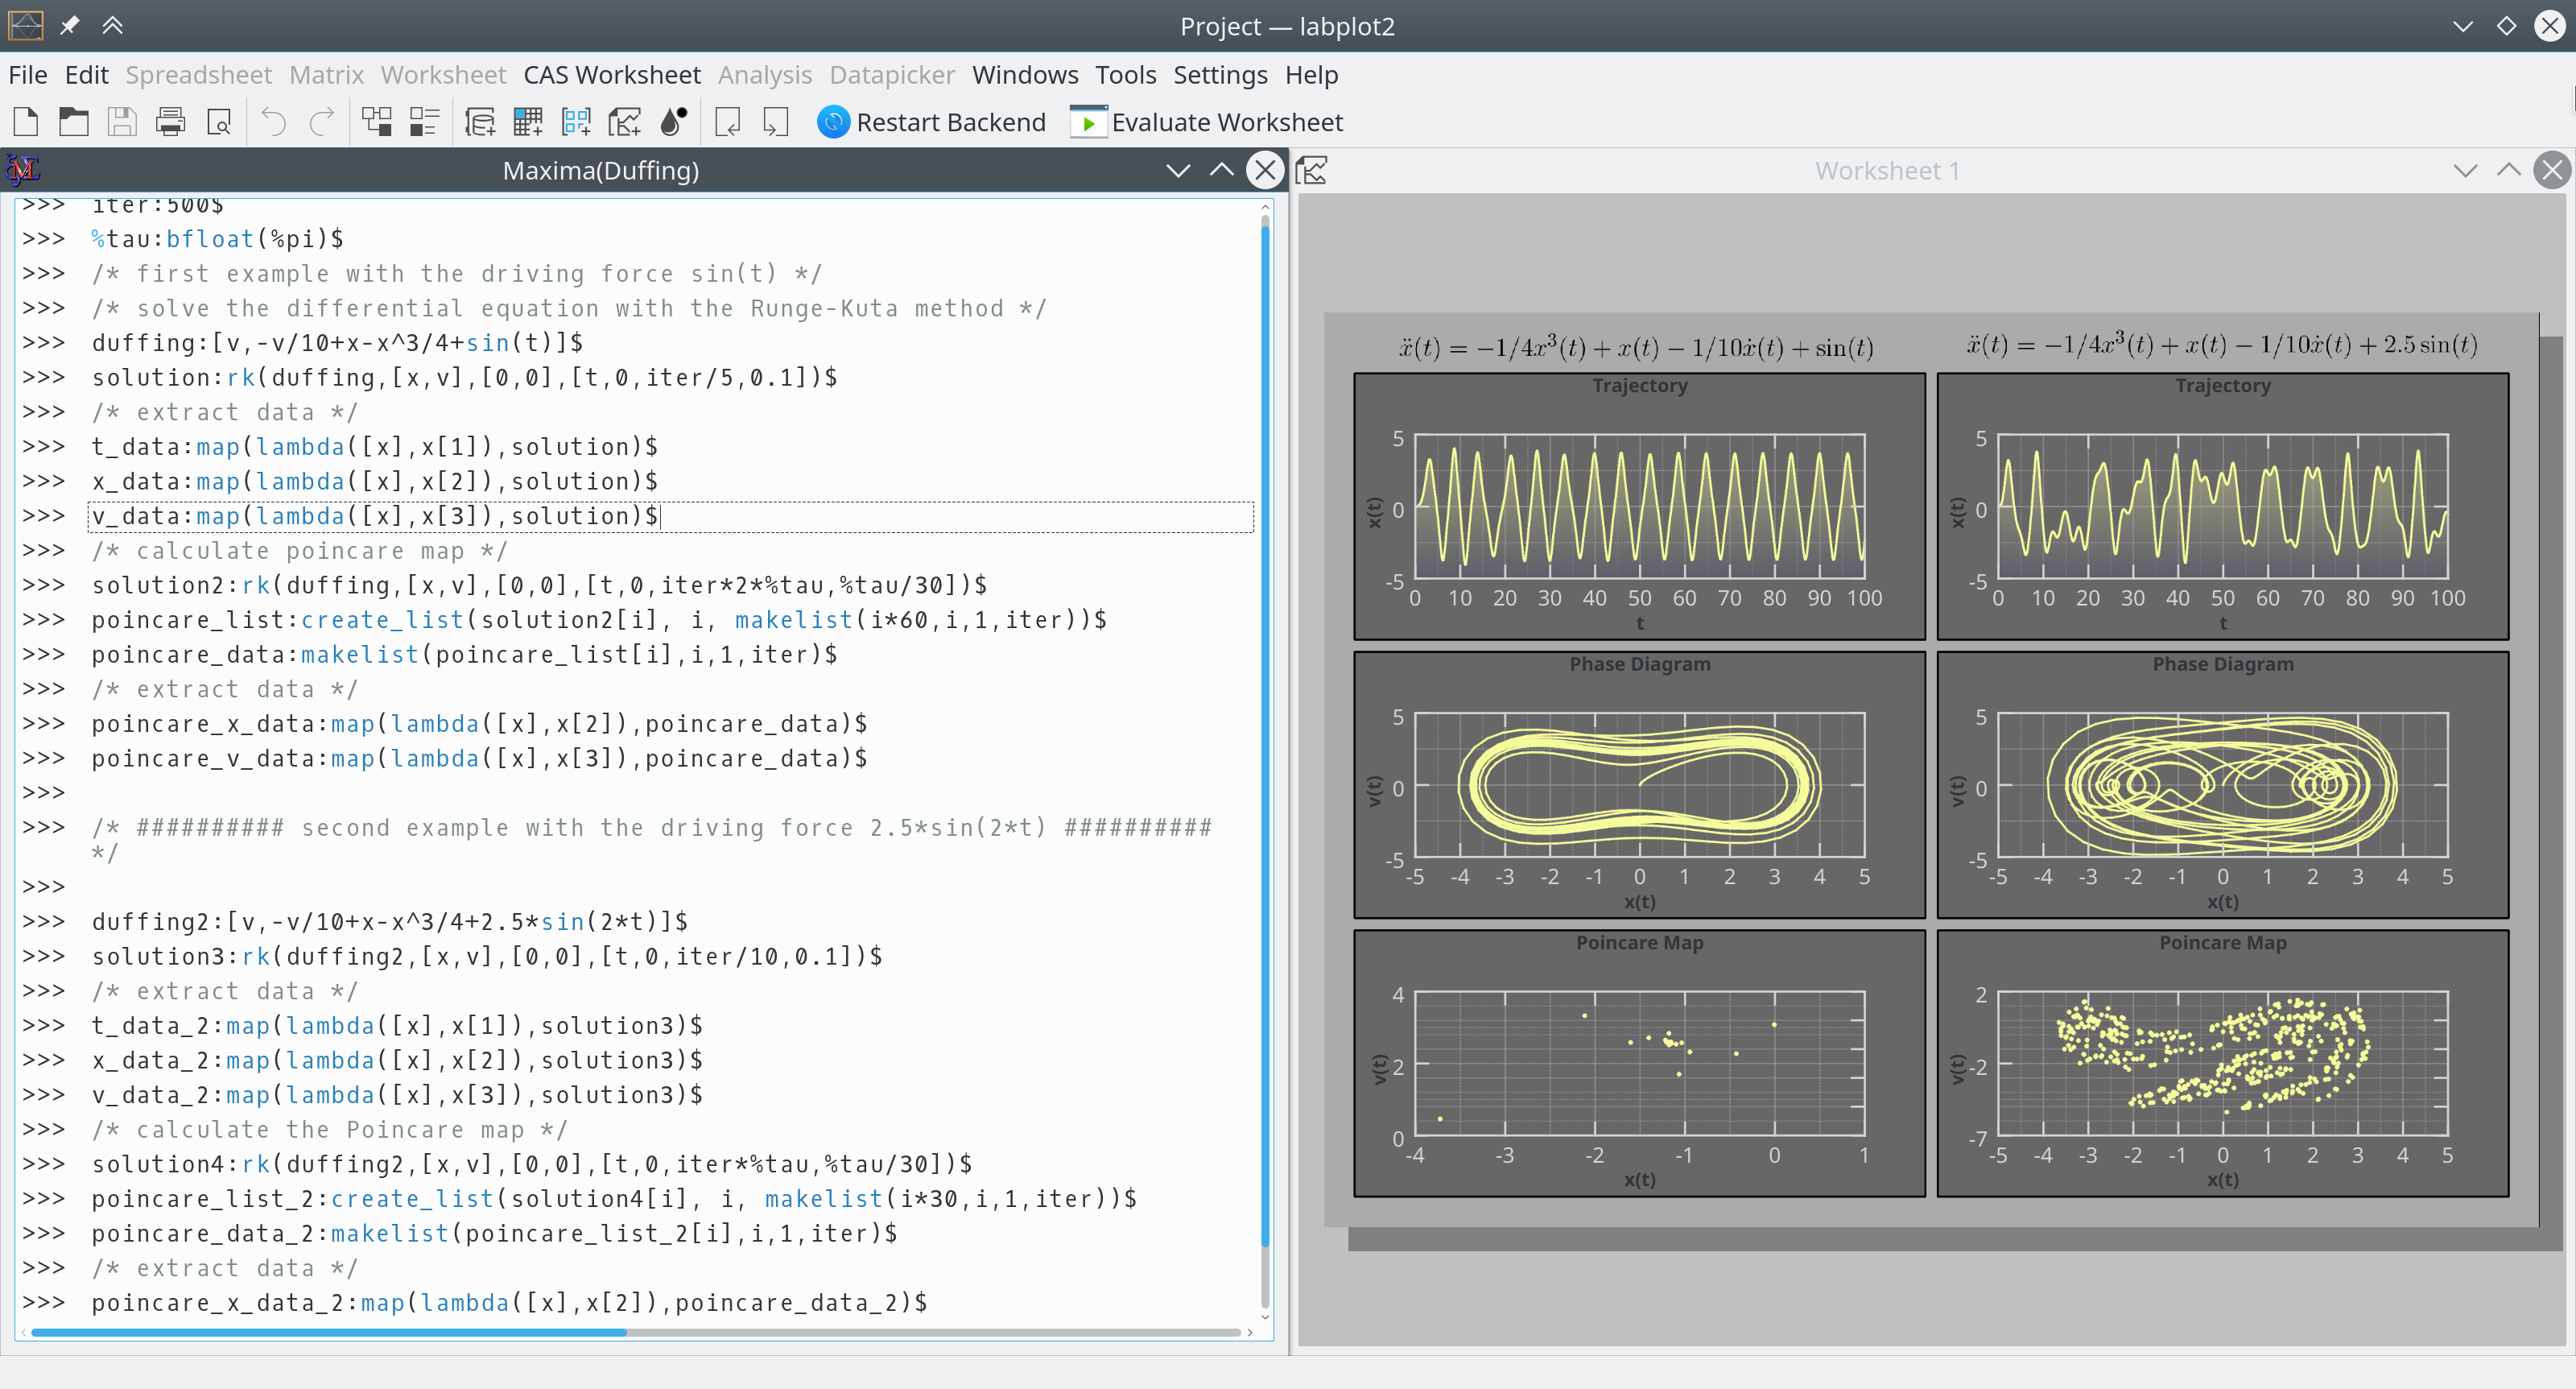
\includegraphics[width=\textwidth]{images/maxima_session.png}
\caption{Maxima session showing the chaotic dynamics of the Duffing oscillator. The differential equation of the forced oscillator is solved with Maxima. Plots of the trajectory, the phase space of the oscillator and the corresponding Poincaré map are done with LabPlot.}
\end{figure}

\begin{figure}
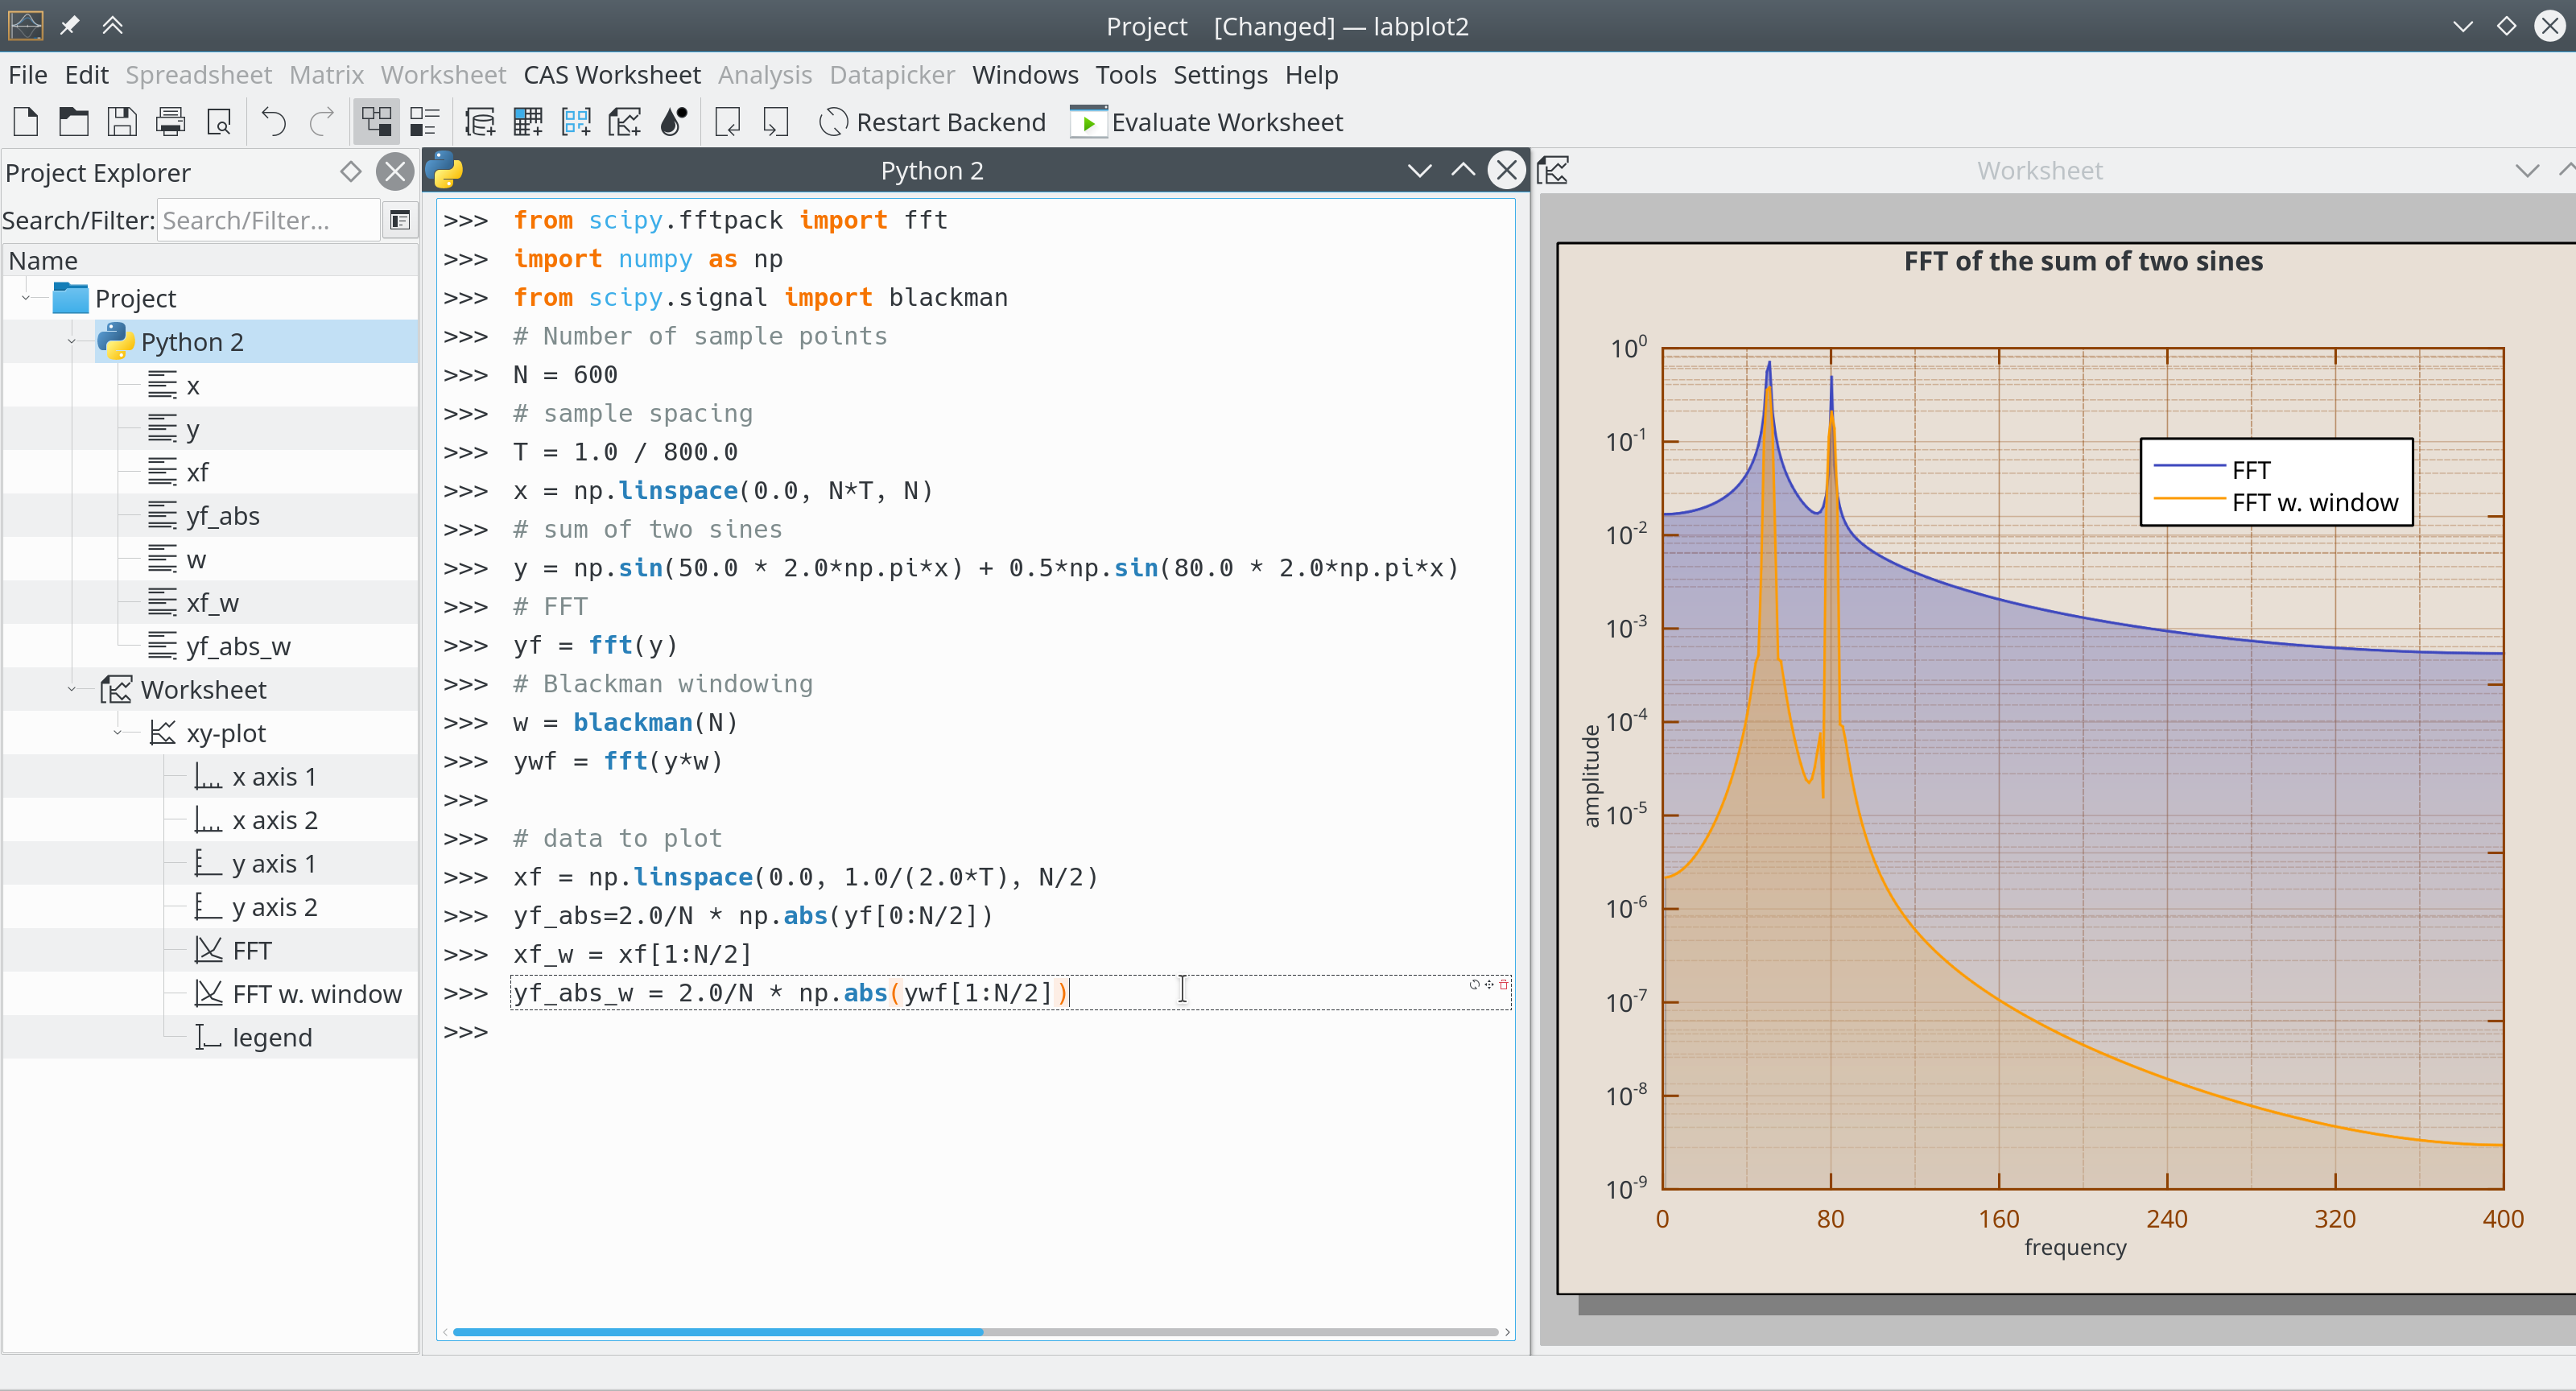
\includegraphics[width=\textwidth]{images/python_session.png}
\caption{Python session illustrating the effect of Blackman windowing on the Fourier transform}
\end{figure}



\chapter{Import and Export}\label{ch:import_export}
\section{Import}\label{sec:import}
\section{Export}\label{sec:export}

\chapter{\LaTeX\, Typesetting}\label{ch:latex_typesetting}
Besides rich text formatting, LabPlot supports \LaTeX\, typesetting in different areas of the application like in text labels, plot title, axis title, etc. In case the \LaTeX\, environment is available on the system (more about the prerequisites below), the user can switch between the \LaTeX\, and rich-text typesettings in the text fields for objects that support this.

In \LaTeX\, mode when entering text in the text field, LabPlot automatically adds a mathematical environment, if not available yet. The user can simply start typing the mathematical expression which will be rendered correctly or, e.g. when combining with text, explicitly specify at which position the mathematical environment has to be used. LabPlot will add the proper header and footer. Following examples are valid inputs
\begin{itemize}
\item {
\begin{lstlisting}
\sum
\end{lstlisting}
}
%
\item {
\begin{lstlisting}
$\sum$
\end{lstlisting}
}
%
\item {
\begin{lstlisting}
\begin{displaymath}
\sum
\end{displaymath}
\end{lstlisting}
}
%
\item {
\begin{lstlisting}
summation symbol $\sum$
\end{lstlisting}
}
\end{itemize}
Furthermore, it is possible to provide a complete \LaTeX\, document
\begin{lstlisting}[language={[Latex]TeX}, backgroundcolor=\color{lightgray}, frame=single]
\documentclass{...}
\begin{document}
...
\end{document}
\end{lstlisting}

With this it is possible to use user-specific header and footer and to include additional packages that are not included by LabPlot on default. This allows to use texts and graphics of arbitrary complexity supported by \LaTeX.

Default rendering engine is, if available, \textit{pdflatex}. In application settings dialog (\menuchoice{Settings}{Configure\, LabPlot}) it is possible to choose between other available rendering engines like \textit{latex, pdflatex, xelatex} or \textit{lualatex}.

To modify the apprearence of the rendered text, the user can specifiy the font size and color. For engines that support OpenType and TrueType fonts (\textit{xelatex} and \textit{lualatex}) it is also possible to provide the main font.


\textbf{Prerequisites:}\\
To render the text set using \LaTeX\, syntax, LabPlot relies on the existence of a \LaTeX\, environment. The rendered document is converted to a PNG image that is imported into and shown in LabPlot. The conversion process depends on the rendering engine used:
\begin{itemize}
\item When using \textit{latex}, the produced DVI file is converted first to a PostScript file with the help of \textit{dvips}. The intermediate PostScript file is converted after that to a PNG file using \textit{convert} from the \textit{ImageMagick} package.
\item For rendering engines producing a PDF file (\textit{pdflate, xelatex} and \textit{lualatex}), the result PDF file is directly converted to a PNG file with \textit{convert}.
\end{itemize}

In case no \LaTeX\, installation is found on the system or one of the required tools for the conversion to PNG is missing, \LaTeX\, typesetting is disabled. On Unix/Linux the required packages are installed via the package manager. The Windows installer for LabPlot and the Mac OS X \textit{dmg}-bundle include already \textit{convert} - everything else has to be installed by the user on the system prior to using this typesetting mode in LabPlot.

When openning a LabPlot project file already containing \LaTeX\, rendered text on systems with no \LaTeX\, typesetting enabled (because of missing prerequisites), the rendered image is  correctly shown but no editing is possible - the user still can switch to the rich-text format mode instead and modify the text.


\textbf{Note about the technical implementation:}\\
The text provided by the user is enriched with an appropriate header and footer to obtain a valid and complete \LaTeX\, document that is processed, as described above, by the rendering engine.
The overall structure of the document generated by LabPlot is
\begin{lstlisting}[language={[Latex]TeX}, backgroundcolor=\color{lightgray}, frame=single, morekeywords={definecolor,color,defaultfontfeatures,setmainfont}]
\documentclass{minimal}
\usepackage{color}
\usepackage[active,displaymath,textmath,tightpage]{preview}
\usepackage{mathtools}
\definecolor{fontcolor}{rgb}{red, green, blue}

%% for xelatex and lualatex engines only
\usepackage{xltxtra}
\defaultfontfeatures{Ligatures=TeX}
\setmainfont[Mapping=tex-text]{font family}
%%

\begin{document}
\begin{preview}
\fontsize{font size}{font size}
\selectfont
\color{fontcolor}

...

\end{preview}
\end{document}
\end{lstlisting}
Here, "red", "green" and "blue" are the font colors provided by the user, "font family" is the OpenType or TrueType font family for the main document font (relevant for xelatex and lualatex only) and "font size" is the size of the font to be used. The text entered by the user, shown as "..." in the listing above, is wrapped into a preview-environment to render the document in a minimal possible size.

In case a complete \LaTeX document is provided, LabPlot merges the definitions of user's header and footer with the definitions shown in the above listing.



\chapter{Tools}\label{ch:tools}
\section{Curve Tracing}\label{sec:curve_tracing}
\textit{Datapicker} is a tool that allows to easily extract data from image files. The process of extraction consists mainly out of the following steps:
\begin{itemize}
\item Import an image containing plots and curves where you want to read the data points from
\item Select the plot type (cartesian, polar, etc)
\item Select tree reference points and provide values for them. With the help of these points the logical coordinate system is determined
\item Create a new datapicker curve and set the type of the error bars.
\item Switch to the mouse mode "Set Curve Points" and start selecting points on the imported image - the coordinates for the selected points are determined and added to the spreadsheet "Data".
\end{itemize}

It is possible to add more than one datapicker curve. This is useful in case the imported image contains several curves that need to be digitized.
The datapicker curve that is currently being selected in the \nameref{sec:project_explorer} is the "active" one - points clicked on the datapicker image will be calculated and added to its data spreadsheet.
\begin{figure}
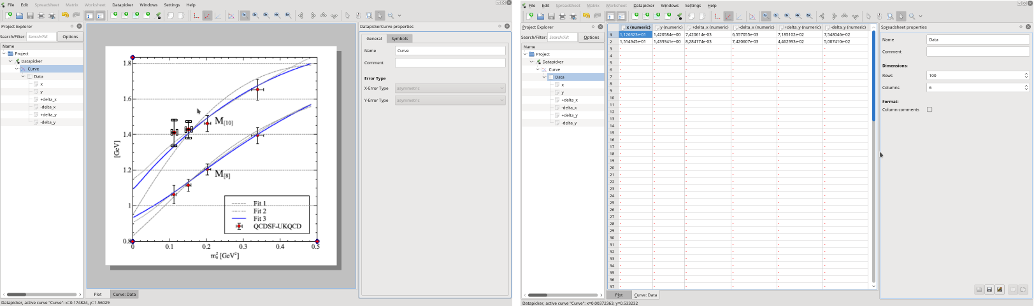
\includegraphics[width=\textwidth]{images/datapicker_active_curve_data_spreadsheet.png}
\caption{Coordinates of the digitized data points stored in a spreadsheet}
\end{figure}

Calculated values are stored in different columns in data spreadsheets in the datapicker. These columns behave exactly the same like other columns
in usual spreadsheets and can be directly used as source columns for curves in the plots.

Datapicker supports the process of the data extraction with several helpers. To place the points more precisely, a magnification glass with different magnification levels is available.
Also, the last selected point can be shifted with the help of the navigation keys.
Furthermore, when reading data points having error bars, datapicker automatically creates bars indicating the end points of the error bars.
Those bars can be pulled with the mouse until the required length (the distance to the data point) is reached.

The procedure for the extraction of data from an imported plot as described above is feasible when dealing with a limited number of points.
In case the curves in the imported image are given as solid lines, the datapicker tool in LabPlot allows to read them semi-automatically.
For this, after a new datapicker curve was added as described above, switch to the mouse mode "Select Curve Segments". The curves on the plot are recognized and highlighted.
By clicking on a highlighted curve (or one of its segments), points along this curve are created.
The length of a segment and the density of created points (separation between two points) are adjustable parameters.
On the screenshots below, after switching to the segment mode all black lines were highlighted (green colour).
In this specific case, the curve was recognized as a single segment and a single mouse-click on this segment is sufficient to digitize this curve and to automatically place points along the curve.
\begin{figure}
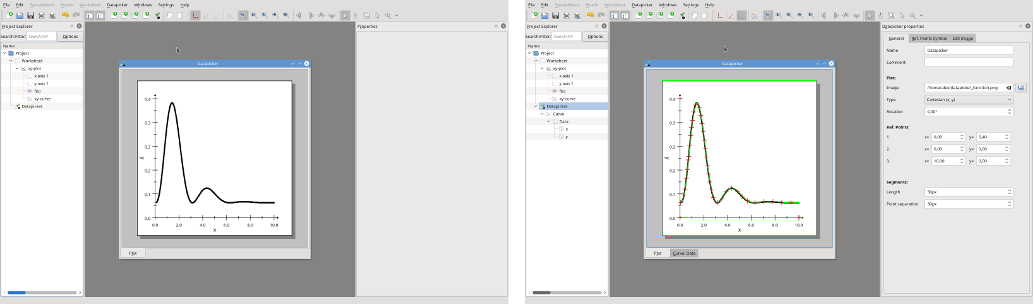
\includegraphics[width=\textwidth]{images/datapicker_segments.png}
\caption{Automatic creation of points along the recognized curve.}
\end{figure}

In many cases the plot is not as simple as above (single black curve on white background) and contains grid lines, many curves of different colour and thinness and a non-white background.
In such a case the automatic detection fails (too many or no objects are highlighted). To help the datapicker to determine the curve(s) correctly, the user has to limit the allowed ranges in the HSV (or HSI) colour spaces.
To subtract the non-white background it is possible to limit the range for the foreground colour, too.
Internally, each pixel of the image is converted to black and white where only the points fitting into the user-defined ranges for hue, saturation, value, intensity and foreground are set to black.

On the screenshots below, the blue curves in the original image were projected onto by having appropriately reduced the allowed ranges in the colour space (note the peak for blue in the histogram for the hue).
The transformed black and white image contains only the curves the user is interested in and it is now an easy task for the datapicker to determine the curves and to place points on them.
\begin{figure}
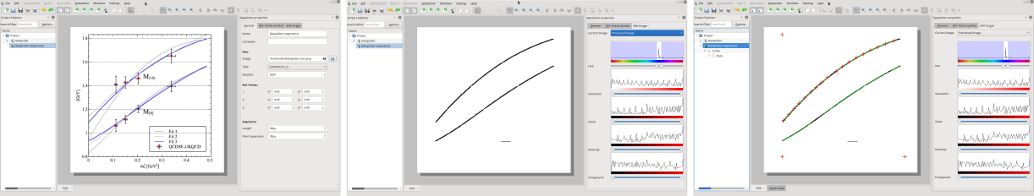
\includegraphics[width=\textwidth]{images/datapicker_original_transformed_segments.png}
\caption{Original image, image with the reduced color space and automatically created points for the recognized curve.}
\end{figure}

Similar to \nameref{sec:worksheet}, the currently visible area in the datapicker can be exported. The supported image formats are described in the section \nameref{sec:export}.


\section{FITS Metadata Editor}
FITS is an open standard file format widely used in the scientific community to store structured as well as unstructured multi-dimenstional data. One of the major features of the FITS format is the ability to store the metadata in human-readable \textit{headers}. Such headers are stored in the file, in addition to the actual data, as key-value pairs in the ASCII format and provide additional information about the origin of the data, its size, used measurement devices, etc. As described in more details in the section \nameref{sec:import}, LabPlot supports the import of data stored in the FITS format. In addition to that, LabPlot also provides the tool \textit{"FITS Metadata Editor"} that allows to inspect and to modify the metadata.

In general, a FITS file consists of one or more \textit{Header + Data Unit}s (HDUs), where the first HDU is usually called the \textit{primary HDU}. A FITS file can have any number of additional HDUs, commonly called FITS \textit{extensions}. LabPlot's FITS Metadata Editor parses the metadata part of the selected FITS file only and shows all available headers (primary and extensional) in a tree view. Already existing key-value pairs can be modified or deleted, new pairs can be added. It is also possible to open and to edit more than one file at the same time.

\begin{figure}
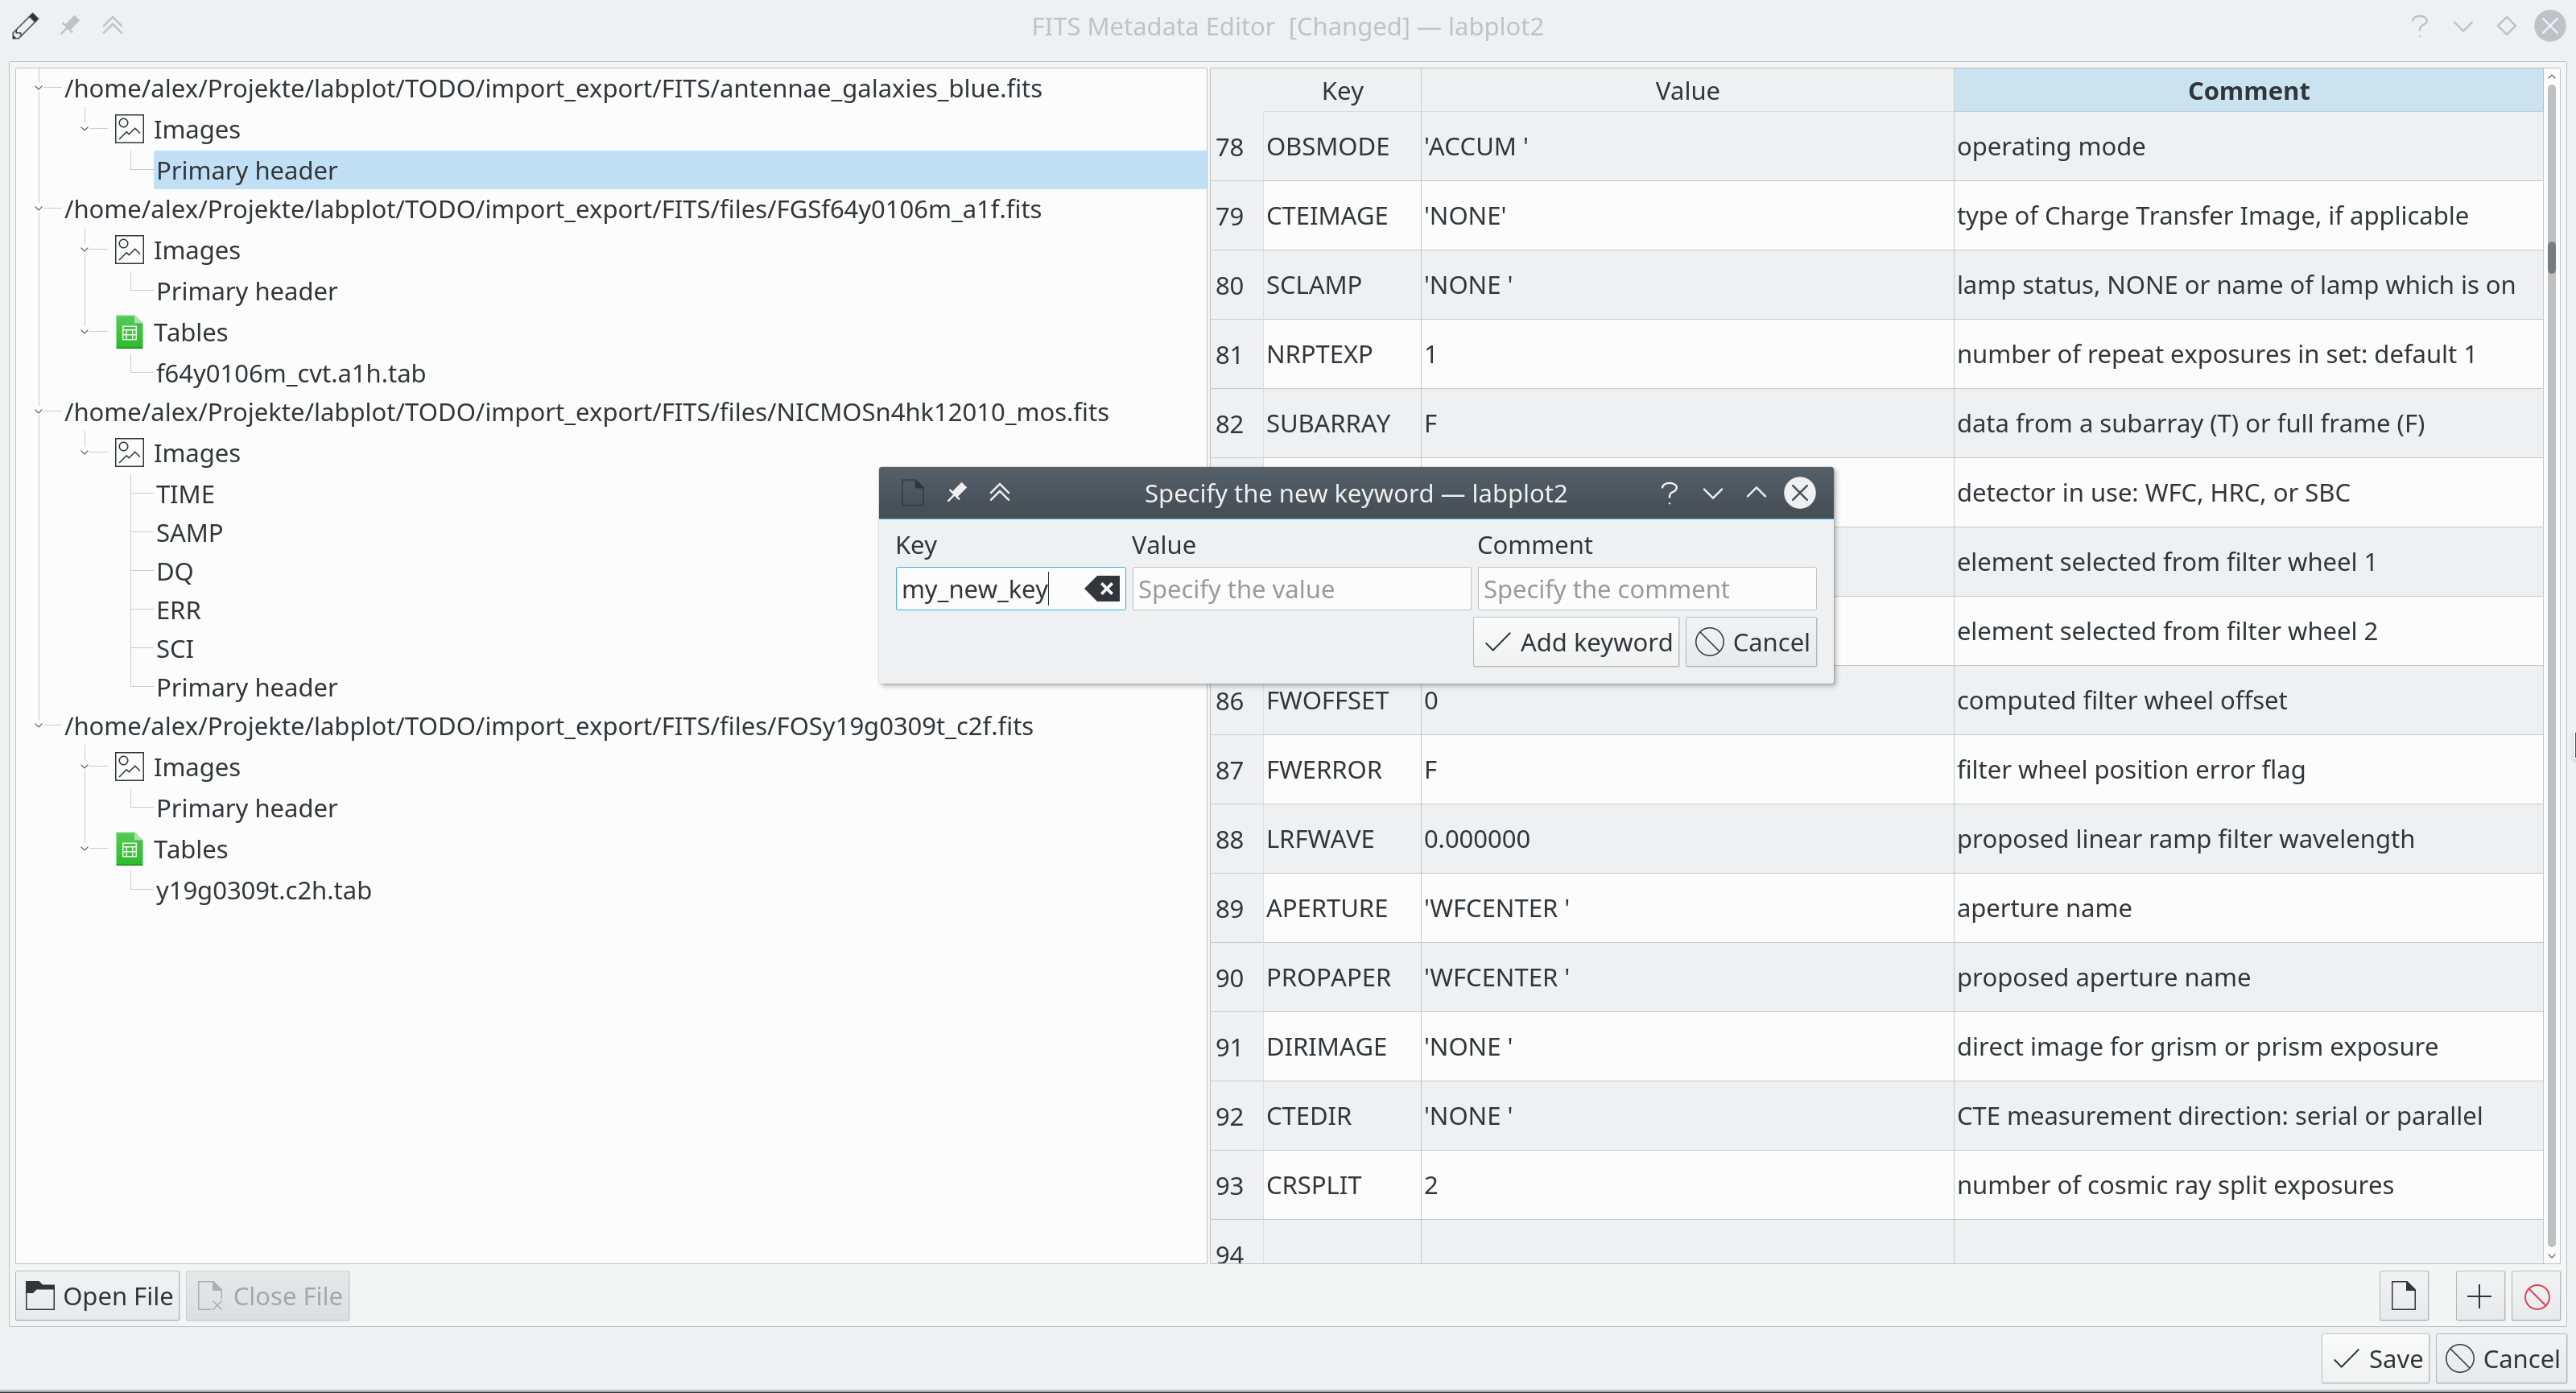
\includegraphics[width=\textwidth]{images/fits_metadata_editor.png}
\caption{FITS Metadata Editor with four opened files and a dialog for adding a new keyword.}
\end{figure}
